\documentclass[11pt, a4paper]{article}
\usepackage{pdfpages}
\usepackage{parallel}
\usepackage[T2A]{fontenc}
\usepackage{ucs}
\usepackage[utf8x]{inputenc}
\usepackage[polish,english,russian]{babel}
\usepackage{hyperref}
\usepackage{rotating}
\usepackage[inner=2cm,top=1.8cm,outer=2cm,bottom=2.3cm,nohead]{geometry}
\usepackage{listings}
\usepackage{graphicx}
\usepackage{wrapfig}
\usepackage{longtable}
\usepackage{indentfirst}
\usepackage{array}
\usepackage{tikzsymbols}
\usepackage{soul}
\usepackage[ruled,vlined]{algorithm2e}
%\counterwithout{figure}{section} 

\usepackage{url}
\makeatletter
\g@addto@macro{\UrlBreaks}{\UrlOrds}
\makeatother

\newcolumntype{P}[1]{>{\raggedright\arraybackslash}p{#1}}
\frenchspacing
\usepackage{fixltx2e} %text sub- and superscripts
\usepackage{icomma} % коскі ў матэматычным рэжыме
\PreloadUnicodePage{4}

\newcommand{\longpage}{\enlargethispage{\baselineskip}}
\newcommand{\shortpage}{\enlargethispage{-\baselineskip}}

\def\switchlang#1{\expandafter\csname switchlang#1\endcsname}
\def\switchlangbe{
\let\saverefname=\refname%
\def\refname{Літаратура}%
\def\figurename{Іл.}%
}
\def\switchlangen{
\let\saverefname=\refname%
\def\refname{References}%
\def\figurename{Fig.}%
}
\def\switchlangru{
\let\saverefname=\refname%
\let\savefigurename=\figurename%
\def\refname{Литература}%
\def\figurename{Рис.}%
}

\hyphenation{admi-ni-stra-tive}
\hyphenation{ex-pe-ri-ence}
\hyphenation{fle-xi-bi-li-ty}
\hyphenation{Py-thon}
\hyphenation{ma-the-ma-ti-cal}
\hyphenation{re-ported}
\hyphenation{imp-le-menta-tions}
\hyphenation{pro-vides}
\hyphenation{en-gi-neering}
\hyphenation{com-pa-ti-bi-li-ty}
\hyphenation{im-pos-sible}
\hyphenation{desk-top}
\hyphenation{elec-tro-nic}
\hyphenation{com-pa-ny}
\hyphenation{de-ve-lop-ment}
\hyphenation{de-ve-loping}
\hyphenation{de-ve-lop}
\hyphenation{da-ta-ba-se}
\hyphenation{plat-forms}
\hyphenation{or-ga-ni-za-tion}
\hyphenation{pro-gramming}
\hyphenation{in-stru-ments}
\hyphenation{Li-nux}
\hyphenation{sour-ce}
\hyphenation{en-vi-ron-ment}
\hyphenation{Te-le-pathy}
\hyphenation{Li-nux-ov-ka}
\hyphenation{Open-BSD}
\hyphenation{Free-BSD}
\hyphenation{men-ti-on-ed}
\hyphenation{app-li-ca-tion}

\def\progref!#1!{\texttt{#1}}
\renewcommand{\arraystretch}{2} %Іначай формулы ў матрыцы зліпаюцца з лініямі
\usepackage{array}

\def\interview #1 (#2), #3, #4, #5\par{

\section[#1, #3, #4]{#1 -- #3, #4}
\def\qname{LVEE}
\def\aname{#1}
\def\q ##1\par{{\noindent \bf \qname: ##1 }\par}
\def\a{{\noindent \bf \aname: } \def\qname{L}\def\aname{#2}}
}

\def\interview* #1 (#2), #3, #4, #5\par{

\section*{#1\\{\small\rm #3, #4. #5}}
\ifx\ParallelWhichBox\undefined%
    \addcontentsline{toc}{section}{#1, #3, #4}%
\else%
\ifnum\ParallelWhichBox=0%
    \addcontentsline{toc}{section}{#1, #3, #4}%
\fi\fi%

\def\qname{LVEE}
\def\aname{#1}
\def\q ##1\par{{\noindent \bf \qname: ##1 }\par}
\def\a{{\noindent \bf \aname: } \def\qname{L}\def\aname{#2}}
}

\newcommand{\interviewfooter}[1]{
\vskip 1em
\noindent \textit{#1}
}


\begin{document}

\title{1986 "--- American Mouse}
\date{}
\maketitle

In 1986, the American Computer and Peripheral company released the American 286 desktop computer, based on the i80286 processor \cite{adv}, and equipped with a mouse called the American Mouse (figure \ref{fig:AmericanPic}). The price of the device in a separate sale was \$125 \cite{review}.

\begin{figure}[h]
    \centering
    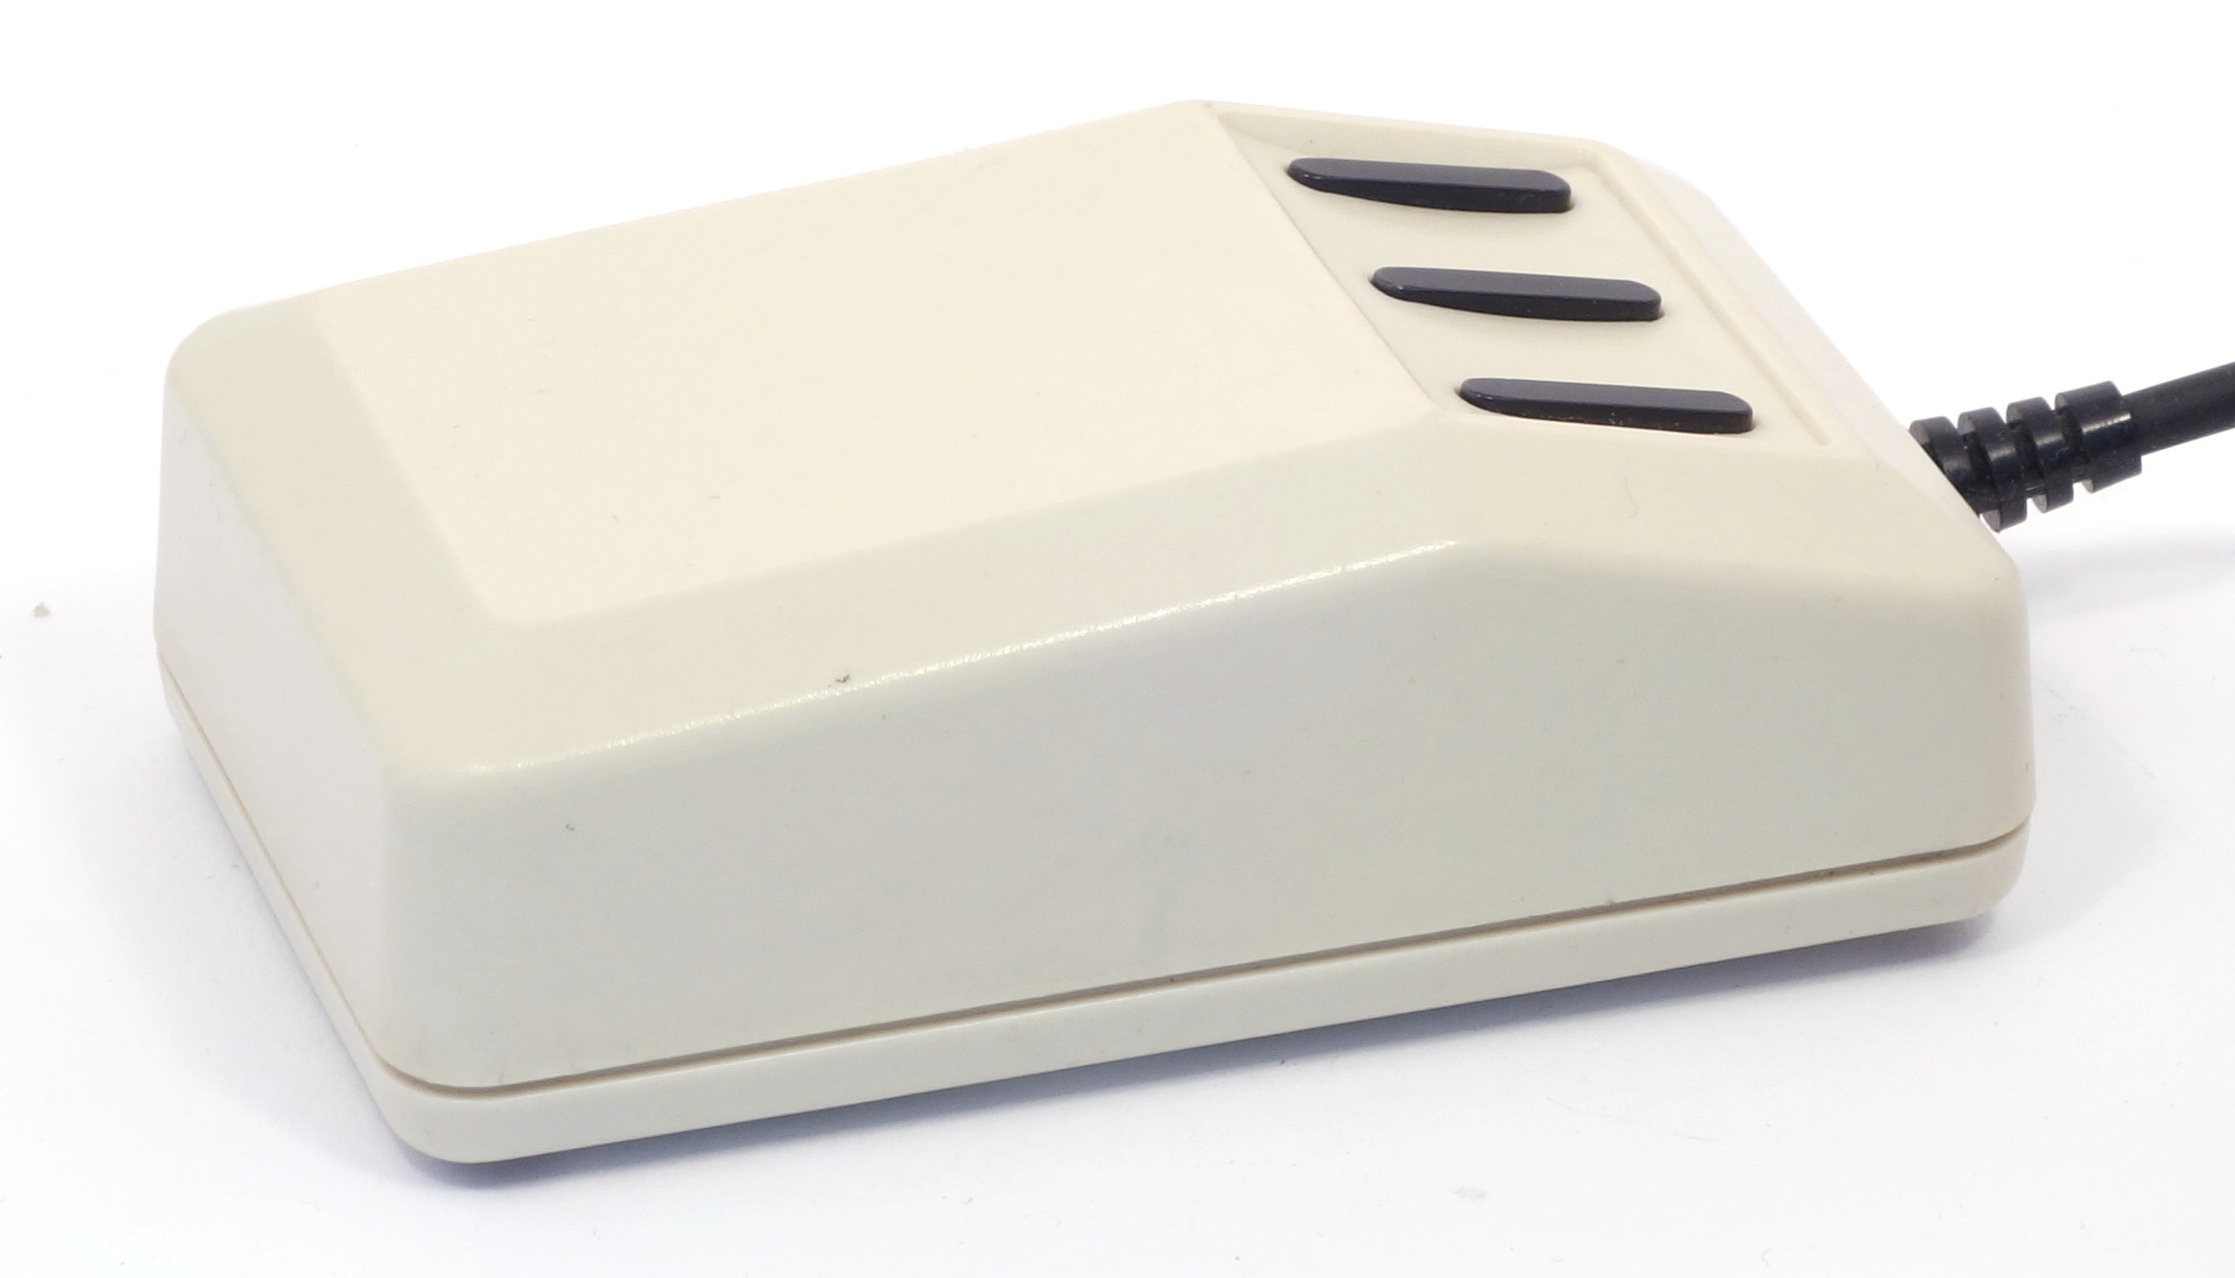
\includegraphics[scale=0.7]{1986_american_mouse/pic_30.jpg}
    \caption{American Mouse}
    \label{fig:AmericanPic}
\end{figure}

A notch on the slightly slanted front of the mouse cover houses three phenomenally narrow buttons. Massive switches located under the buttons forced developers to use an asymmetrical layout of the mouse cable that runs between the left and middle buttons (figure \ref{AmericanTopAndBottom}). The underside of the housing contains a removable ring to remove the ball and clean the mouse. There are no inscriptions or emblems on the case.

\begin{figure}[h]
    \centering
    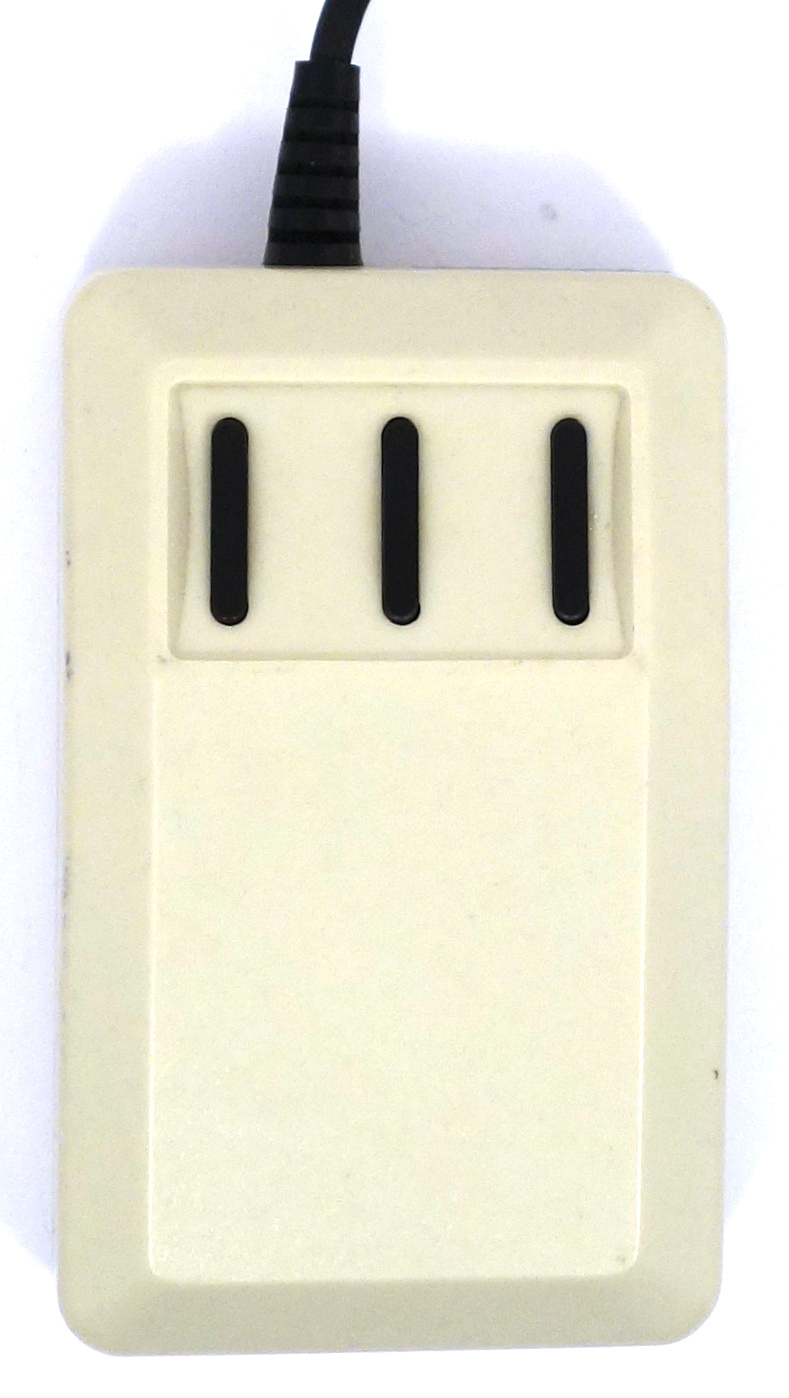
\includegraphics[scale=0.7]{1986_american_mouse/top_60.jpg}
    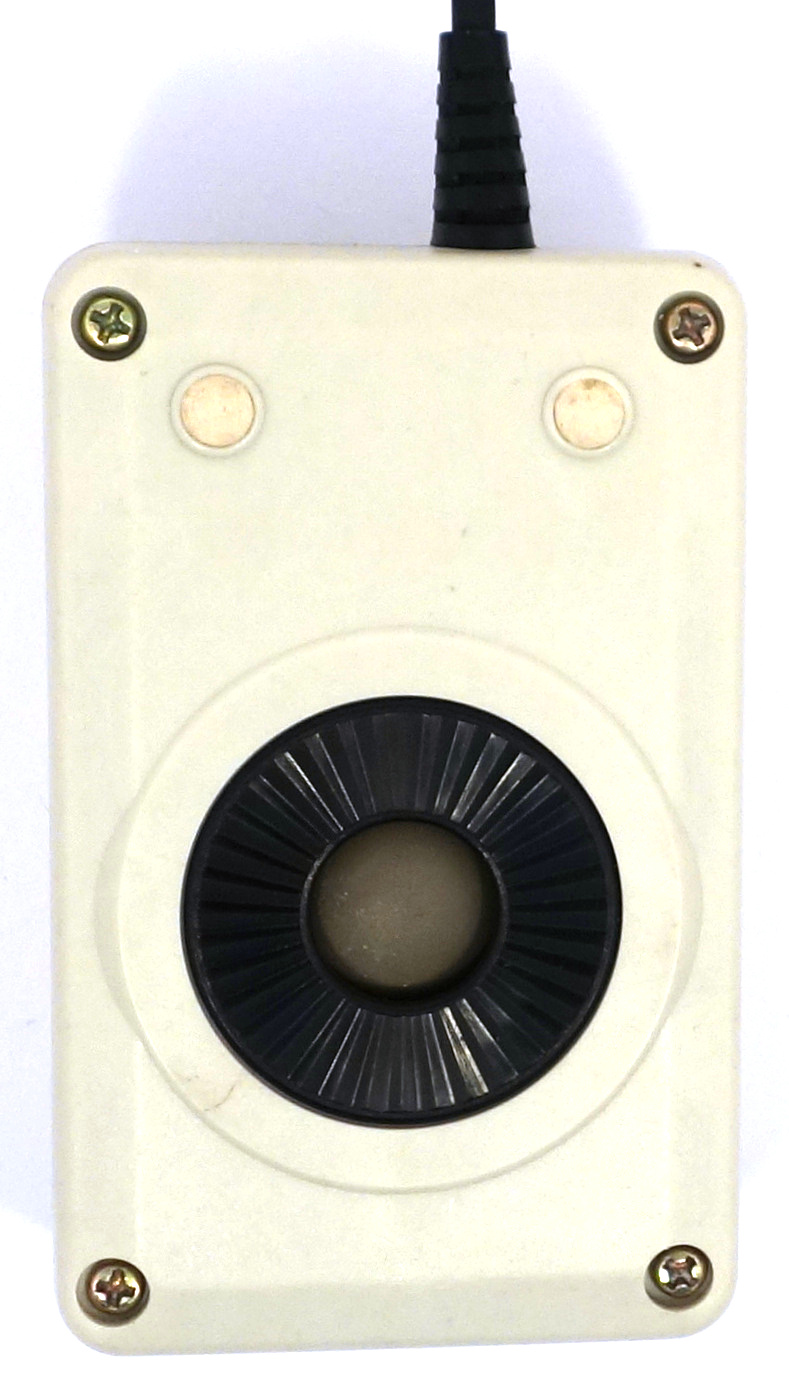
\includegraphics[scale=0.7]{1986_american_mouse/bottom_60.jpg}
    \caption{American Mouse, top and bottom views}
    \label{AmericanTopAndBottom}
\end{figure}

In term of size, the manipulator is an optomechanical cursor control device typical of the 1980s (figure \ref{fig:AmericanSize}).

\begin{figure}[h]
    \centering
    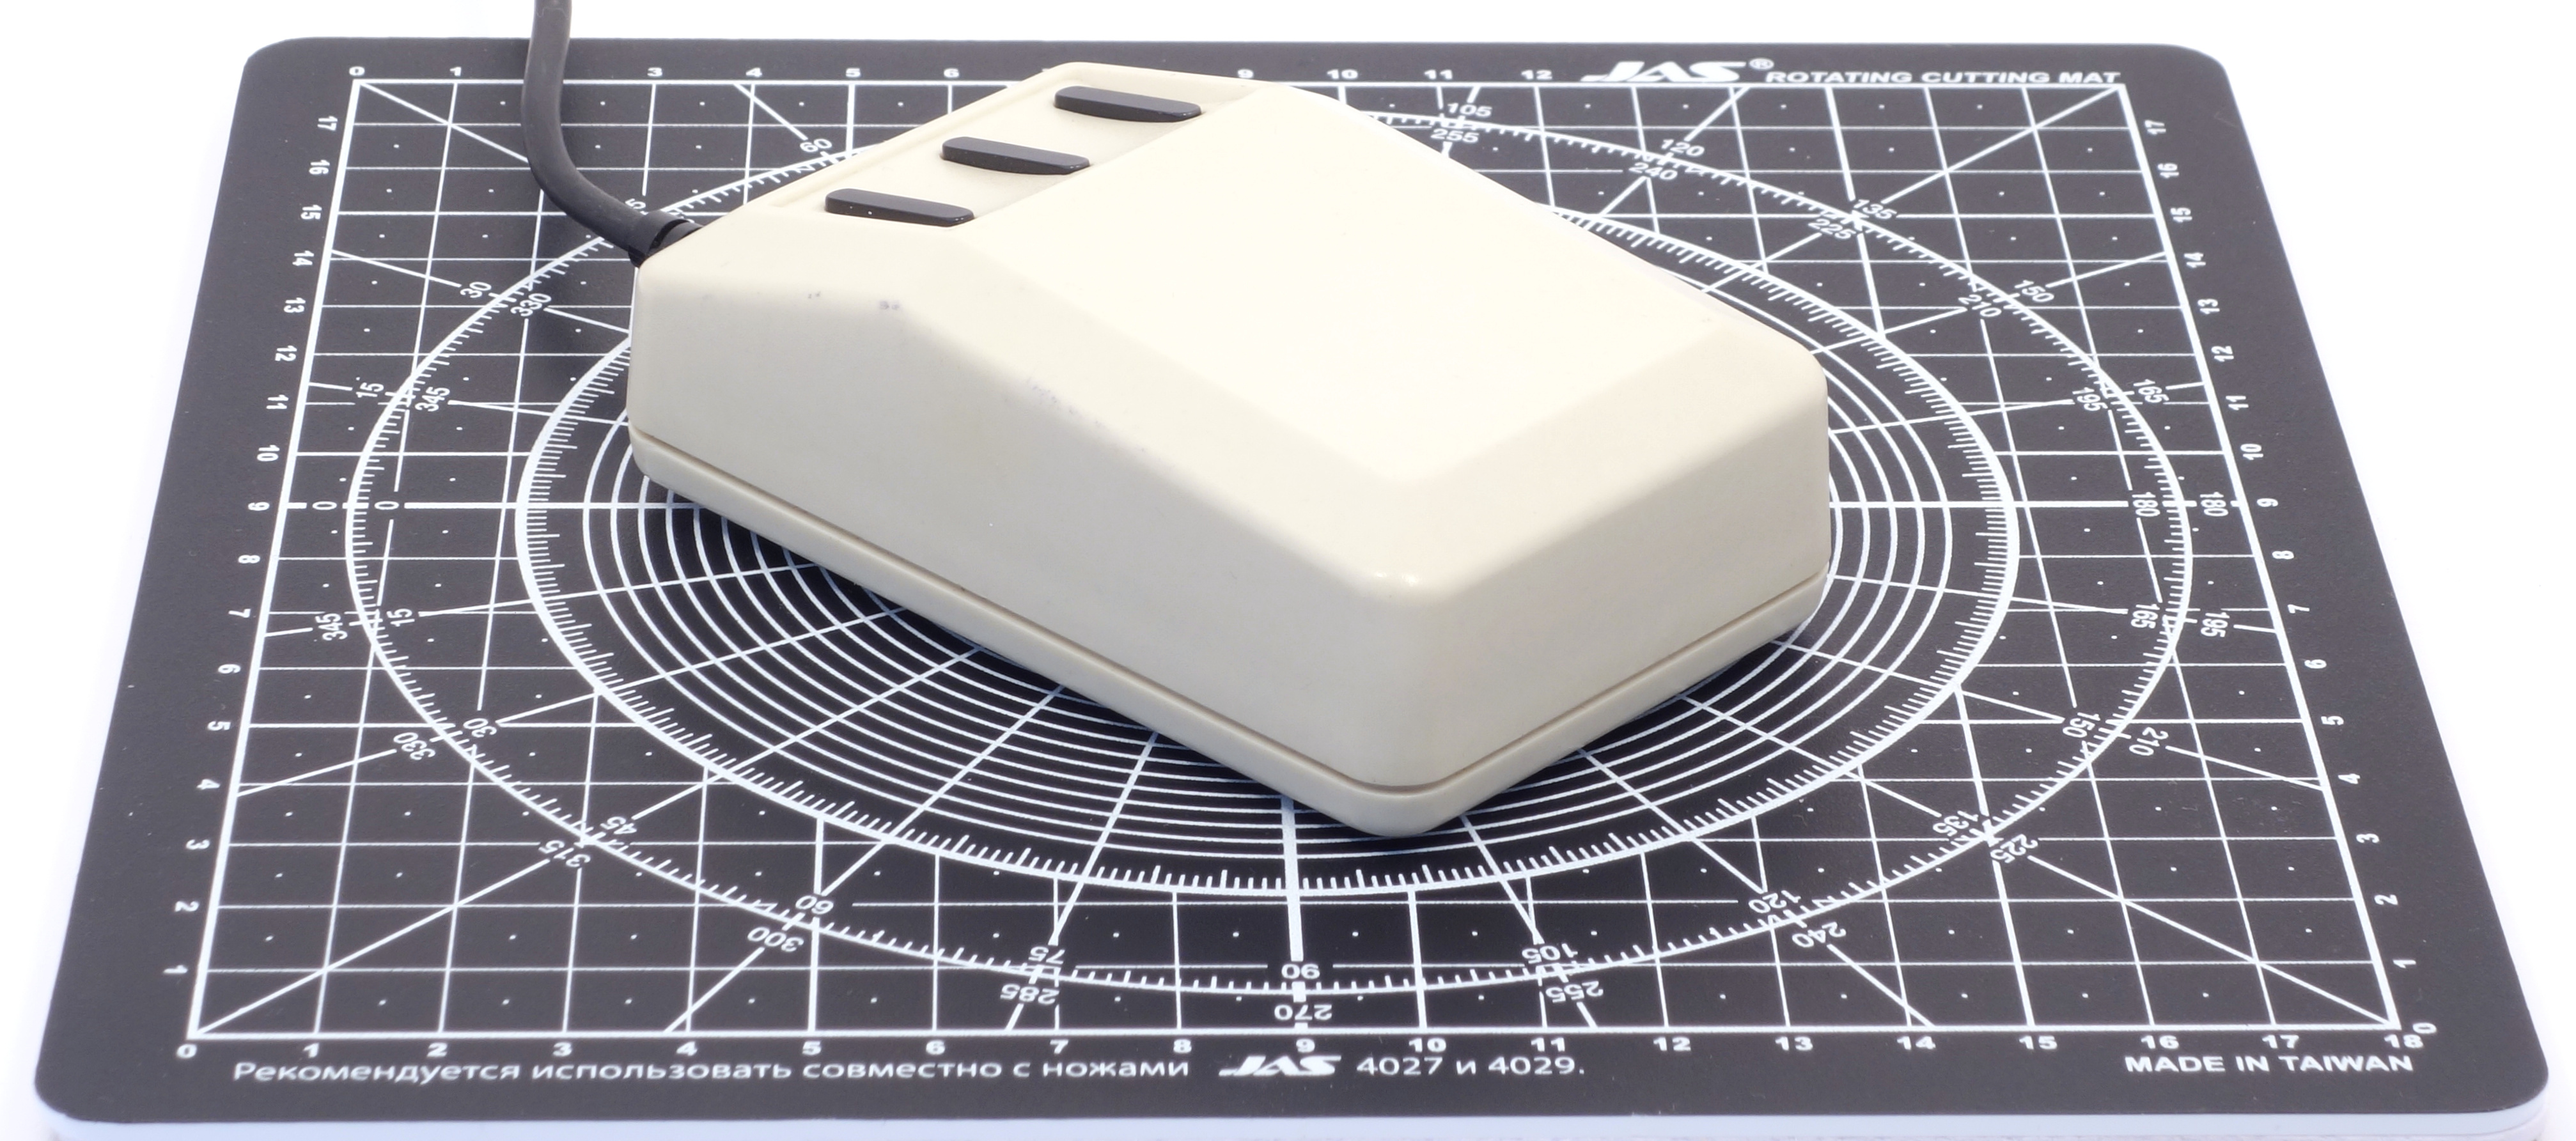
\includegraphics[scale=0.5]{1986_american_mouse/size_30.jpg}
    \caption{Изображение American Mouse on a graduated pad with a grid step of 1~cm}
    \label{fig:AmericanSize}
\end{figure}

The exterior of the American Mouse has a clear industrial design. At the same time, the angular body was equipped with beveled edges to provide a more comfortable palm position; however, the need to press extremely narrow buttons that cut into the fingertips negates the ergonomic efforts of the developers and allows us to rank this manipulator among the most questionable devices in the design (figure \ref{fig:AmericanHand}).

\begin{figure}[h]
    \centering
    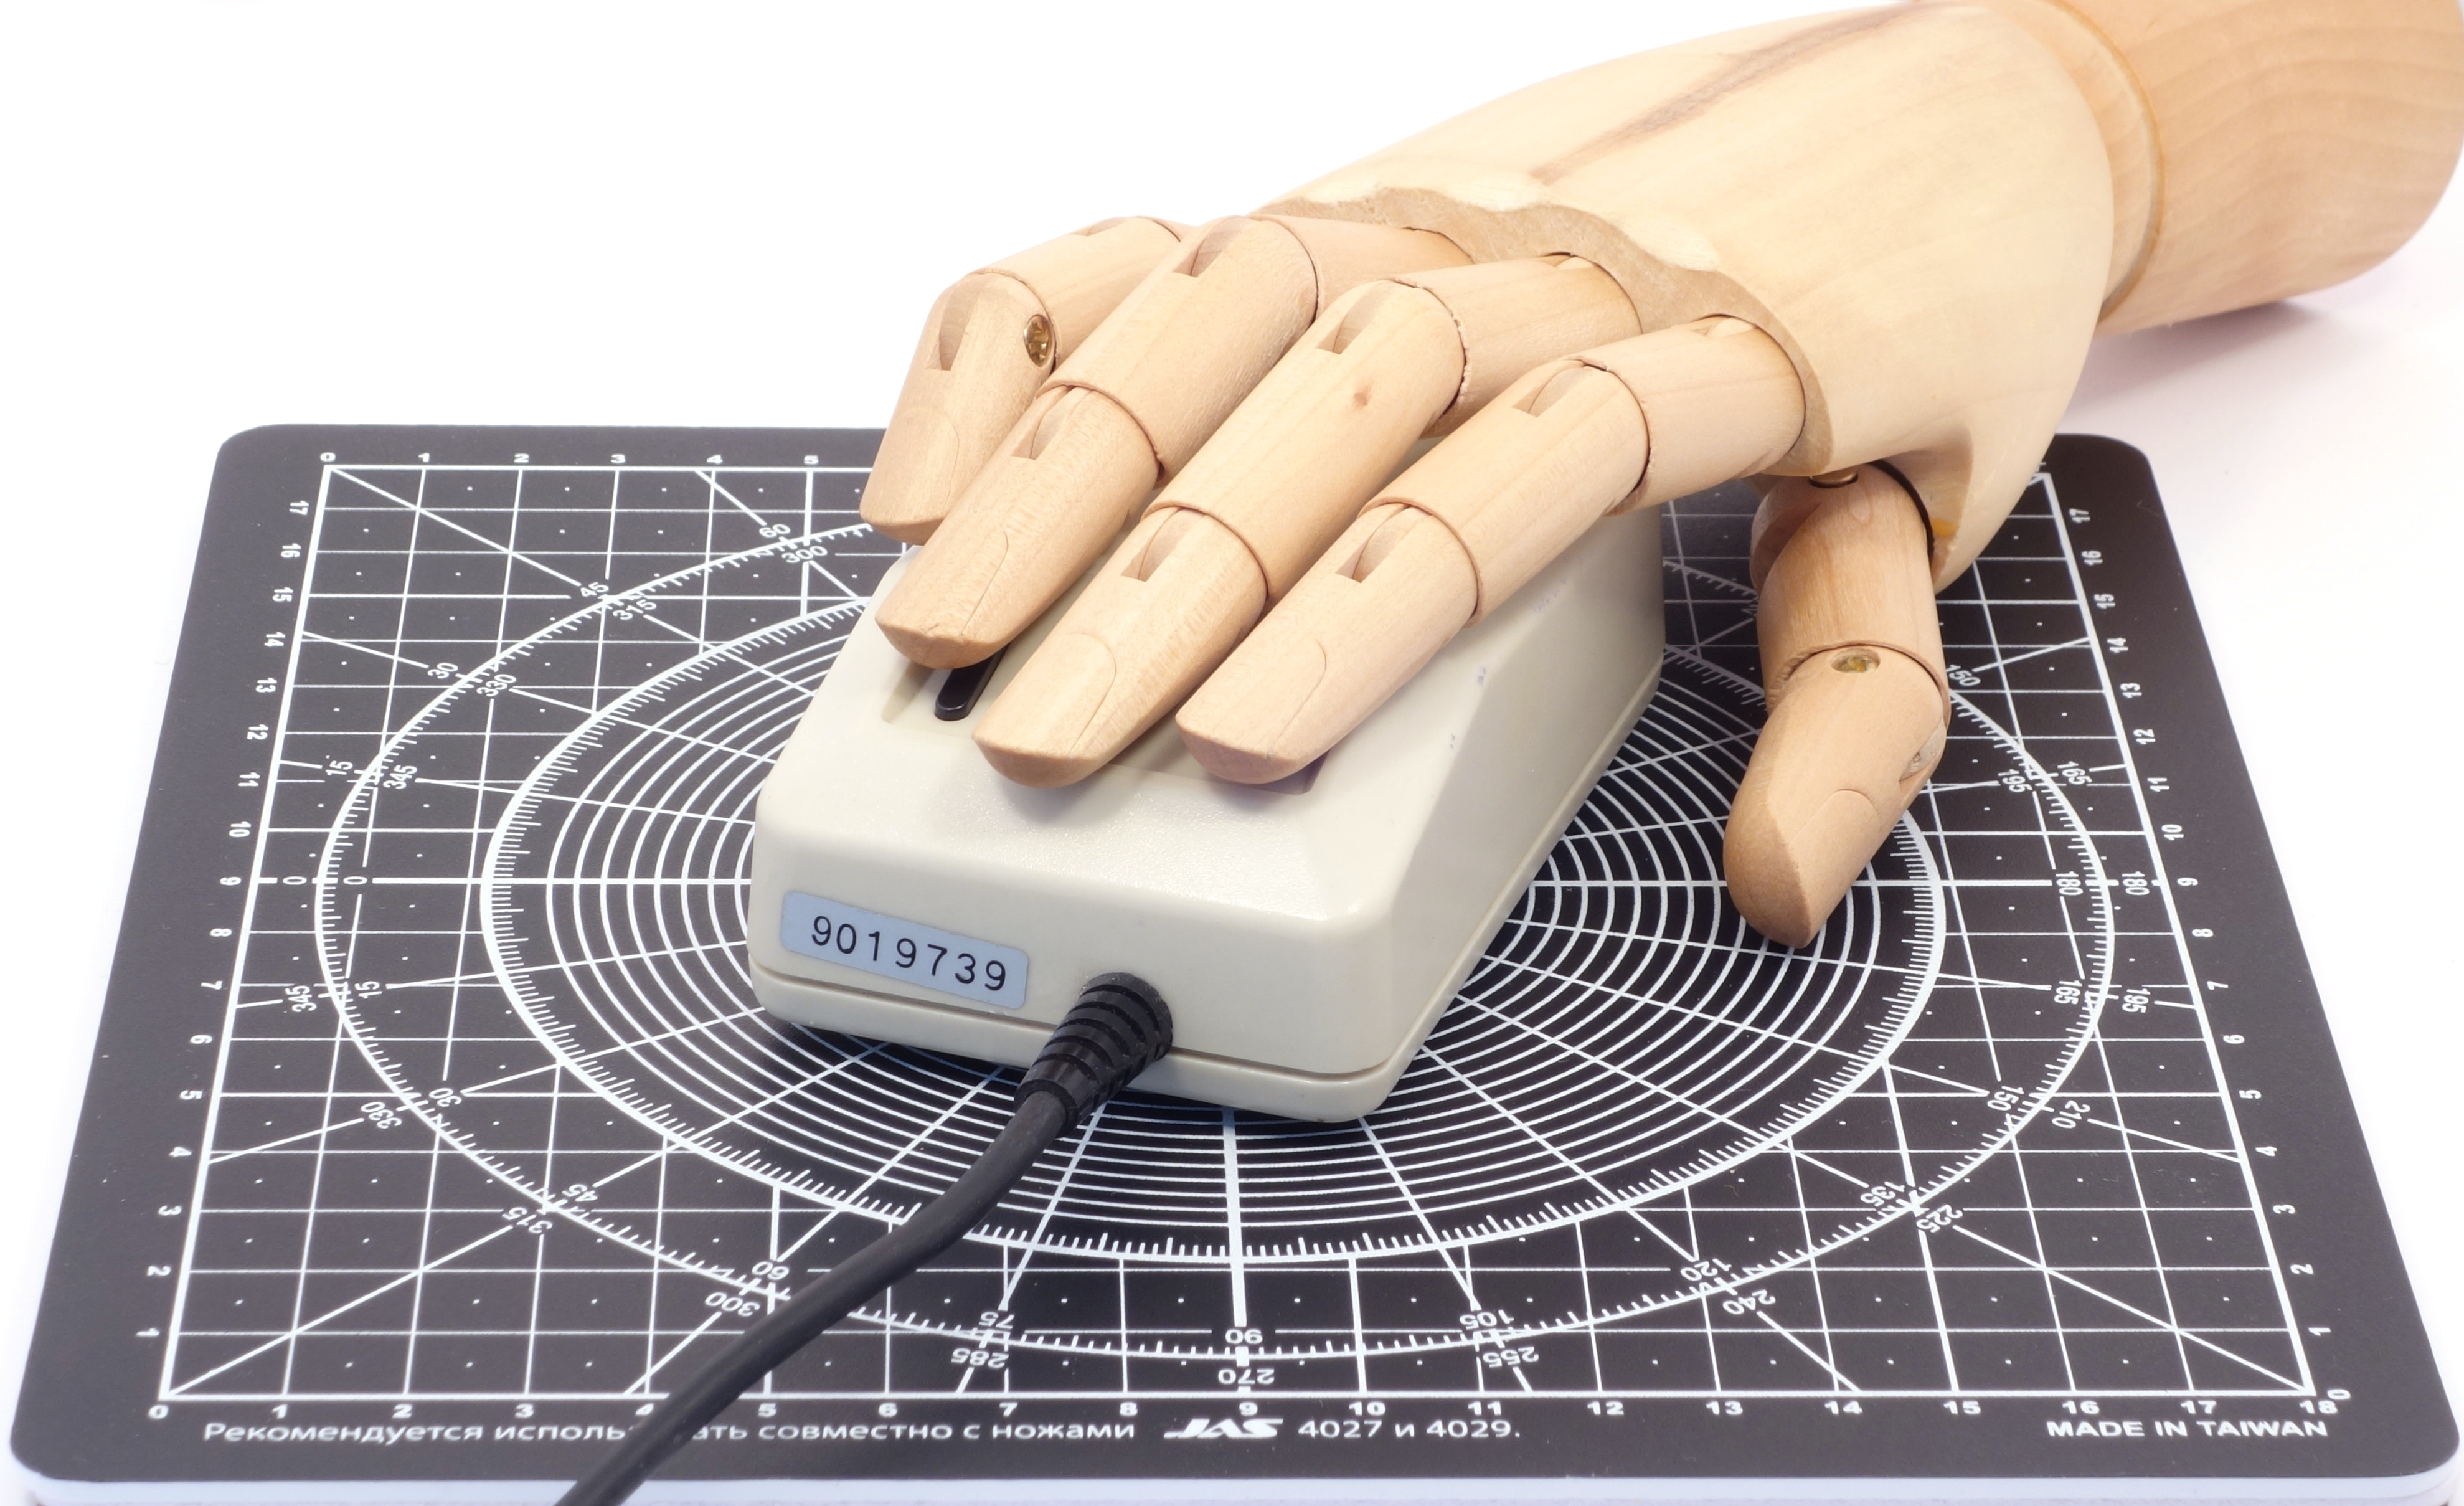
\includegraphics[scale=0.5]{1986_american_mouse/hand_30.jpg}
    \caption{American Mouse with a human hand model}
    \label{fig:AmericanHand}
\end{figure}

The Americanl Mouse has a D-SUB connector and an RS-232 interface. The device follows the Mouse Systems protocol, however this is not mentioned in the accompanying brochure. And when this mouse was on the market, the driver for this protocol could be found mainly bundled with Mouse Systems optical mice, which limited the possibility of using the American Mouse with third-party software. The only software package that came with the mouse was Compu-Brush, a rebranded PC Paint program.

\begin{figure}[h]
    \centering
    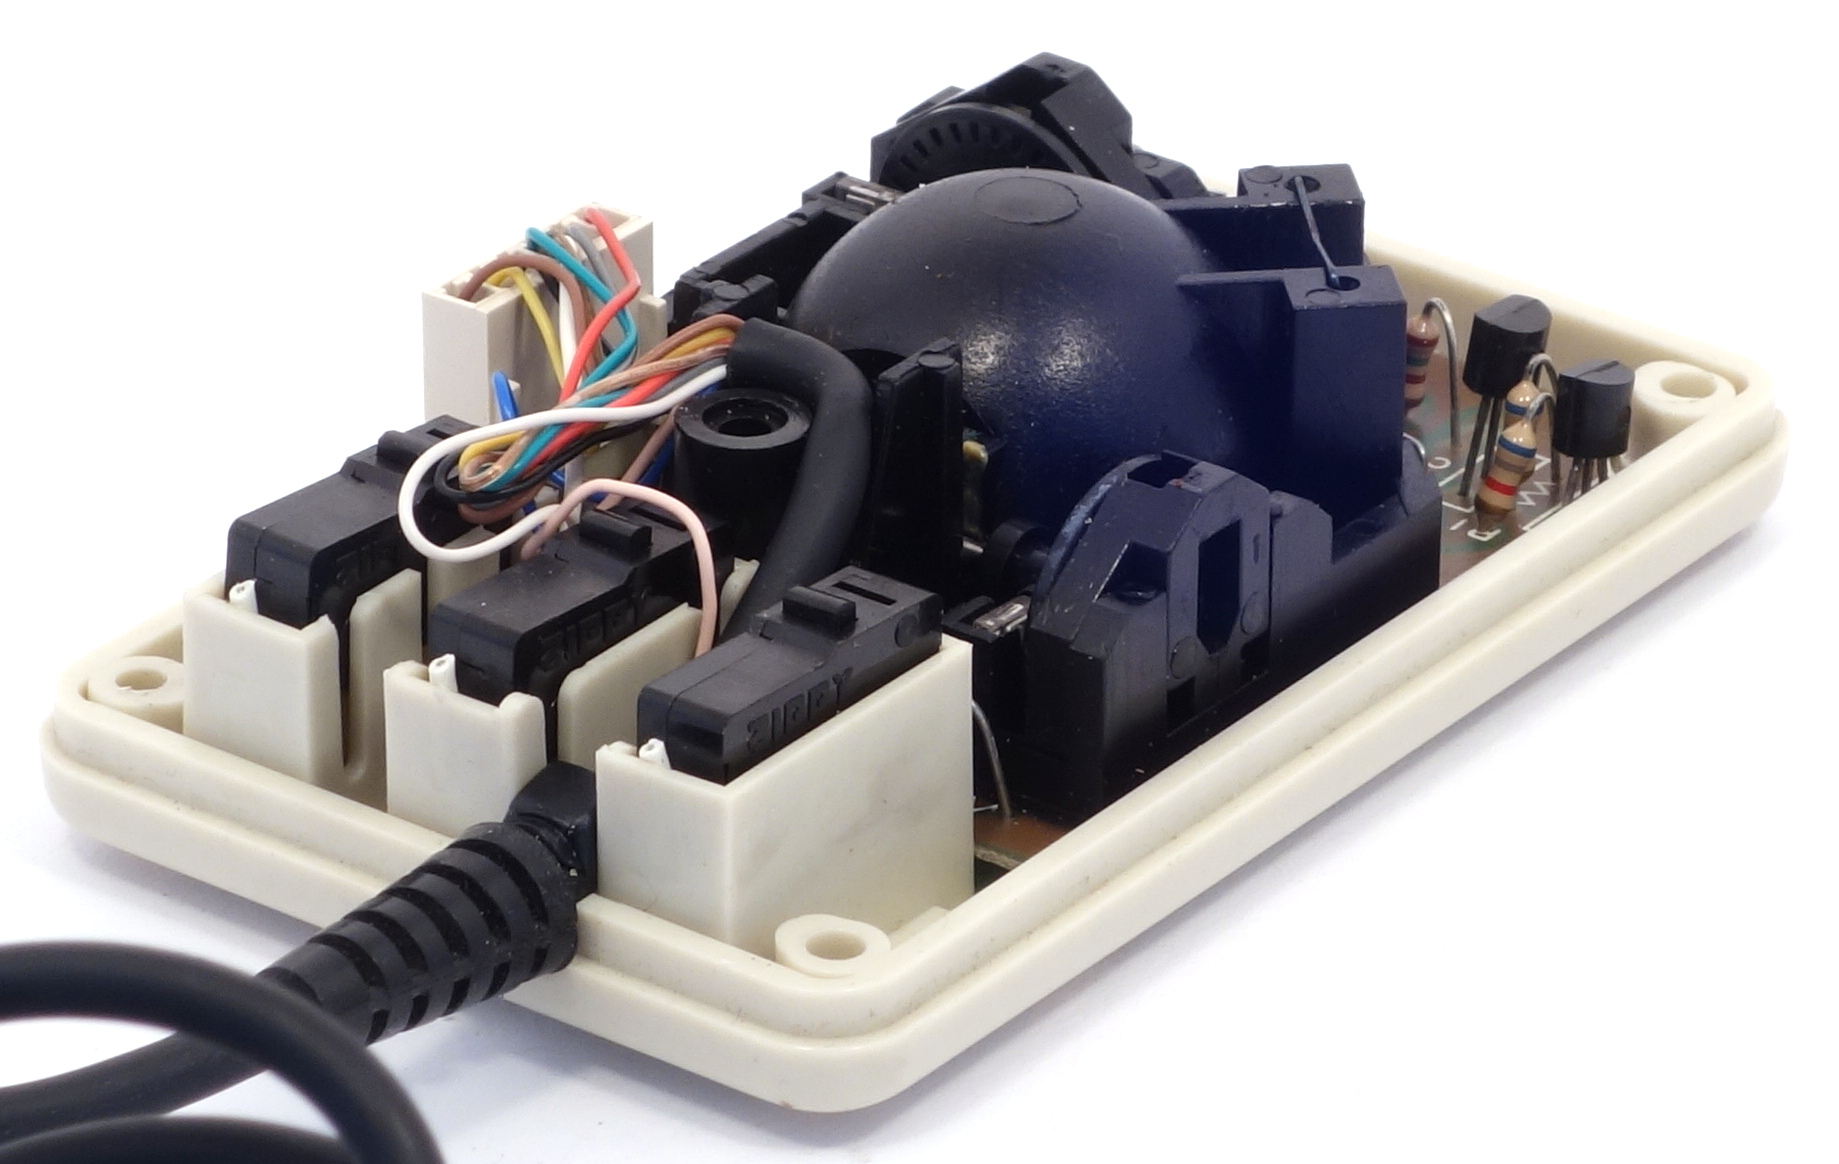
\includegraphics[scale=0.9]{1986_american_mouse/inside_60.jpg}
    \caption{American Mouse disassembled}
    \label{fig:AmericanInside}
\end{figure}

Trackball internals are shown on figure \ref{fig:AmericanInside}. The figure shows a fairly standard design of the opto-mechanical mouse. Worthy of mention is the dense filling of the internal space of the case with various plastic details that are absent in almost hollow optmechanical mice of a later period.

\begin{thebibliography}{9}
\bibitem {adv} I love American (advertising). // PC MAGAZINE, V. 5, No. 18. October 1986, p. 157. \url{https://archive.org/details/PC-Mag-1986-10-28/page/n159}
\bibitem {review} Barr Ch. Mice for mainstream applications // PC MAGAZINE, V. 6, No. 14., August 1987, pp. 119 – 146 \url{https://archive.org/details/PC-Mag-1987-08-01/page/n121}
\end{thebibliography}
\end{document}
